\documentclass{sig-alt-release2}
\usepackage{url}
\usepackage{color}
\usepackage{graphics,graphicx}
\usepackage{subfigure}

\usepackage{aeguill}

\usepackage{epsfig}
\usepackage{epstopdf}

\usepackage{colortbl}
\usepackage{multirow}
\usepackage{booktabs}
\usepackage{ifthen}  

\usepackage{array}

\begin{document}
\newcommand{\todo}[1]{\textcolor{red}{#1}}
\def\newblock{\hskip .11em plus .33em minus .07em}

\conferenceinfo{DIM3} {2012, Glasgow, UK} 
\CopyrightYear{2012}
\clubpenalty=10000
\widowpenalty = 10000

\title{{Where in the BOB?}}

\numberofauthors{4}
\author{
Andrei Palade, 0907350, 0907350p@student.gla.ac.uk\\
Andrei Mustata, 0907390, 0907390m@student.gla.ac.uk\\
Cristian Urlea, 1102465, 1102465u@student.gla.ac.uk \\
Wei Zhang, 1104733, 1104733z@student.gla.ac.uk\\
\\
          \affaddr{\textbf{Group F, DIM3}}\\
    %  \affaddr{Dim3}\\
%      \affaddr{Student no.s}\\
 %            \email{\{ 0907350, 0907390, 1102465, 1104733\}
  %           @students.glasgow.ac.uk }
}

\maketitle

\begin{abstract}

\textbf{Where in the BOB?} is a simple web application that enables users to
find the location of a room in the Boyd Orr Building. 

The application aims to provide a room search interface to the user.
Results are returned along with a relevant floor plan highlighted to
indicate the particular room.

Our interface also provides relevant lists of room names in case of an ambiguous 
identifier being passed as a query and the ability comment on a particular room. 

\end{abstract}

\section{Aim of Application}

The application name is ``Where in the BOB'' and its purpose is to provide
students, lecturers and visitors of University of Glasgow with an identifying
system of rooms located in Boyd Orr Building. The application intends to
offer an interface where a particular user has the options to view a particular 
room from a floor plan perspective, to view details pertaining to that room and 
leave comments or ratings for it.

The objective, in this case, is to build such a system based on existing 
floor plans of the building. Furthermore, the search facilities are
restricted to a given number of well known room names amongst students
(e.g. Level 3 Computer Science lab) as well as their official names(e.g. Room
720). In this case, if the room is identified, the result of the search will
contain a floor plan with the location of the room highlighted, details
about the room (e.g. number of seats, other details of access, comments on the
room), otherwise it will return a message notifying the user that the search 
process has failed to identify the queried roomroom (i.e. The rooms was not identified).

\subsection{Goals}
Another goal is to provide the user with a list of room names in case that
there are multiple rooms across campus especially in the Boyd Orr Building.
A particular goal which will provide the user with a consistent and optimized
results is to:
\begin{itemize} \itemsep1pt \parskip0pt \parsep0pt
	\item  search again in case of not found 
	\item  leave feedback
	\item  comment on room 
\end{itemize}


\subsection{Assumptions}

We made a number of assumptions based on the purpose of this web application. 
It is assumed that users have at least a bare minimum understanding of the English
language and the required skills to utilise a web browser  as well as having 
an Internet connection.

The visual interaction with the application makes it necessary for the user to 
be able to see and to use one hand in order to interact with the device as they 
do with other applications. This include holding a mouse in order to move a 
pointer around the screen or using fingers to point to different parts of the 
screen on touch-screen hand-held devices.

Another assumption we made is that users will be students or visitors with 
minimal knowledge about the campus and they use their hand-held device for 
coordination around campus.

\subsection{Constraints}

\subsubsection{Development constraints}

The major constraint we are concerned about is the time necessary to develop 
the application. We will use the available time during the labs to implement 
the required functionality of our system and we will also make use of Django 
web framework for fast development. Due to budgetary constraints we are forced 
to use open source software which cause another issue in terms of technical 
knowledge regarding the tools used.

\subsubsection{Application constraints}
\begin{itemize} \itemsep1pt \parskip0pt \parsep0pt
	\item \textbf{End-user environment}: The end-user system can be deployed
	on a wide range of devices (e.g. desktop or mobile systems). These devices
	come with a restricted screen size.
	\item \textbf{Network}: The number of simultaneous connection to the server
	might be bounded by the server capabilities.
\end{itemize}



\subsection{Functionality}
The required and desired functionality of our application is as follows:
\begin{itemize} \itemsep1pt \parskip0pt \parsep0pt
	\item The required functionality:
	\begin{itemize} \itemsep1pt \parskip0pt \parsep0pt
		\item Accept textual search terms and return results for a searched
		room identifier 
		
		\item Provide a graphical view of the room that is being searched
		within Boyd Orr Building
		
		\item Return an SVG format of the floor plan where the searched
		room is located with the room highlighted
		
		\item Return a list of matching results for ambiguous defined
		identifiers
		
		\item Allow users to leave comments for a the searched room		
	\end{itemize}

	\item The desired functionality:
	\begin{itemize} \itemsep1pt \parskip0pt \parsep0pt
		\item Allow users to see the floor map directory
		\item Allow users to search give feedback on the application
		\item Allow users to return and search for a different room
		\item Allow users to check the accessibility of the room
	\end{itemize}
\end{itemize}

\section{Client Interface}

\subsection*{User classes}
This section presents a use case analysis of the website. The use cases 
presented here model the interaction between users and the application.

We have identified the need for two user classes:

\subsubsection*{Visitor}
Visitors are the \textbf{end-users} of the application. They could be either
new students who are not used to the University's campus yet, or anyone else
who can't find their way through the complex system of rooms and hallways that
is the Boyd Orr Building.

\emph{``I'm a level 2 CS student and I can't find my way to the lab. All 
I know is I should be in the \guillemotleft Level 2 lab in the Boyd Orr
\guillemotright. Now, I've managed to find the \textbf{floor}, but I'm not sure
which room I need to go to. Oh,look! There's a room directory up on the wall, 
but it's not very helpful. I sure wish there was an app for this, lol!''}

His goal is to find information regarding a particular room (e.g.: what floor 
it is on, where exactly it is on that floor, etc). He might know the room 
number or some other unofficial name for that room.

They can ask the application about different rooms in the BOB. If that room 
name exists, the app shows an image with the appropriate floor plan and the 
searched room is highlighted.

\subsubsection*{Administrator}
Someone needs to manage all that data, so there will be an administrator. He is
responsible for maintaining the database, ie: adding/removing rooms, floors,
floor plans and the labels for them. They can also edit the comments.

\subsubsection*{User matrix}
The user matrix lists all the functionalities available to each of the user
classes.

\begin{tabular}{| p{4cm} | c | c |} \hline
\textbf{Functionality} & \textbf{Visitor} & \textbf{Admin} \\ \hline
Browse directory & X & X \\ \hline
Search for a room & X & X \\ \hline
Post comment & X & X \\ \hline
Send feedback & X & X \\ \hline
Edit/Delete Comment & & X \\ \hline
Add/edit floor &  & X \\ \hline
Add/edit room & & X \\ \hline
Add/edit floor plan & & X \\ \hline
\end{tabular}	

\subsection*{Walkthrough}
The front page of the app is the ``Home'' page. In order for the users to 
find a room, they can either browse through the ``Rooms and floors
directory'' or they can enter their query in the ``Search box'' provided.

This ``directory'' contains a list of all the existent floors and rooms (each
with link to its own page). While the main functionality of the application is
the ability to search, this directory will also be provided, in case a
user does not know the room by \emph{name}, but knows where the room is \emph{
located}.

By going with the search box, there is a possibility that the room searched by
the user either doesn't exist, or the name is ambiguous, in which case a list
of all the relevant rooms, ie. that are named similarly, is provided.
If there is an exact match, the page for that particular room is displayed.

Once the user gets to a page of a room, a large floor map is provided, with
the searched room being highlighted. All the rooms have labels, so people can
search for the adjacent rooms, once they are on that level.

When clicking on a room area on the floor-plan, a tool-tip appears, showing 
whatever information there is available regarding that room (e.g.: other known
names, type of the room, link to the room's page, etc.). Another option for
displaying this would have been to do it on hovering over that area, but the 
application is also intended to be used with hand-held devices, which have different
pointer behaviours than, say, a desktop PC with a mouse.

\subsection*{Wireframes}
We have tried to design a user interface that is very intuitive, making it
easy for the users to find what they're looking for.

All the pages will have the basic layout of the \textbf{Home} page
(Figure \ref{img:wireframes-home}), which consists of:
\begin{center}
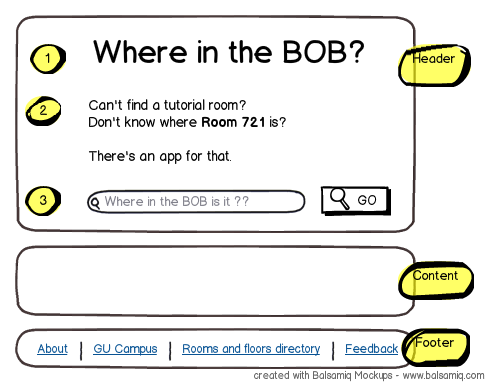
\includegraphics[scale=0.55]{img/wireframes/home2.png}
\end{center}
\begin{itemize} \itemsep1pt \parskip0pt \parsep0pt
	\item{
		\textbf{Header}
		\begin{enumerate} \itemsep1pt \parskip0pt \parsep0pt
			\item{
				\textbf{Name} of the website
			}
			\item{
				\textbf{Tagline}/short description of how the application works, so
				the users won't have to go through the tedious process of
				reading through an \textbf{About} page
			}
			\item{
				\textbf{Search box} - this is where the users input their
				query
			}
		\end{enumerate}
	}

	\item{
		\textbf{Content} - the rest of the page will be displayed in this area
	}
	
	\item{\textbf{Footer} - contains the links for the \textbf{navigation menu}
	}
\end{itemize}


\begin{center}
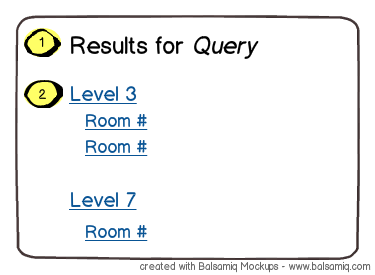
\includegraphics[scale=0.5]{img/wireframes/results.png}
\end{center}


The pages \textbf{Results} and \textbf{Directory} share the same design (Figure 
\ref{img:wireframes-results}): a list of all the levels, and for each one of 
them, a list of rooms. If a query returns more than one result, this page is 
shown with the list of matching rooms. In the case of the Directory page, all 
the levels are listed. Their elements are:
\begin{enumerate} \itemsep1pt \parskip0pt \parsep0pt
	\item{\textbf{Query} - the searched term}
	\item{\textbf{Result set} - the results of the query grouped by the level
	they're on}
\end{enumerate}


\begin{center}
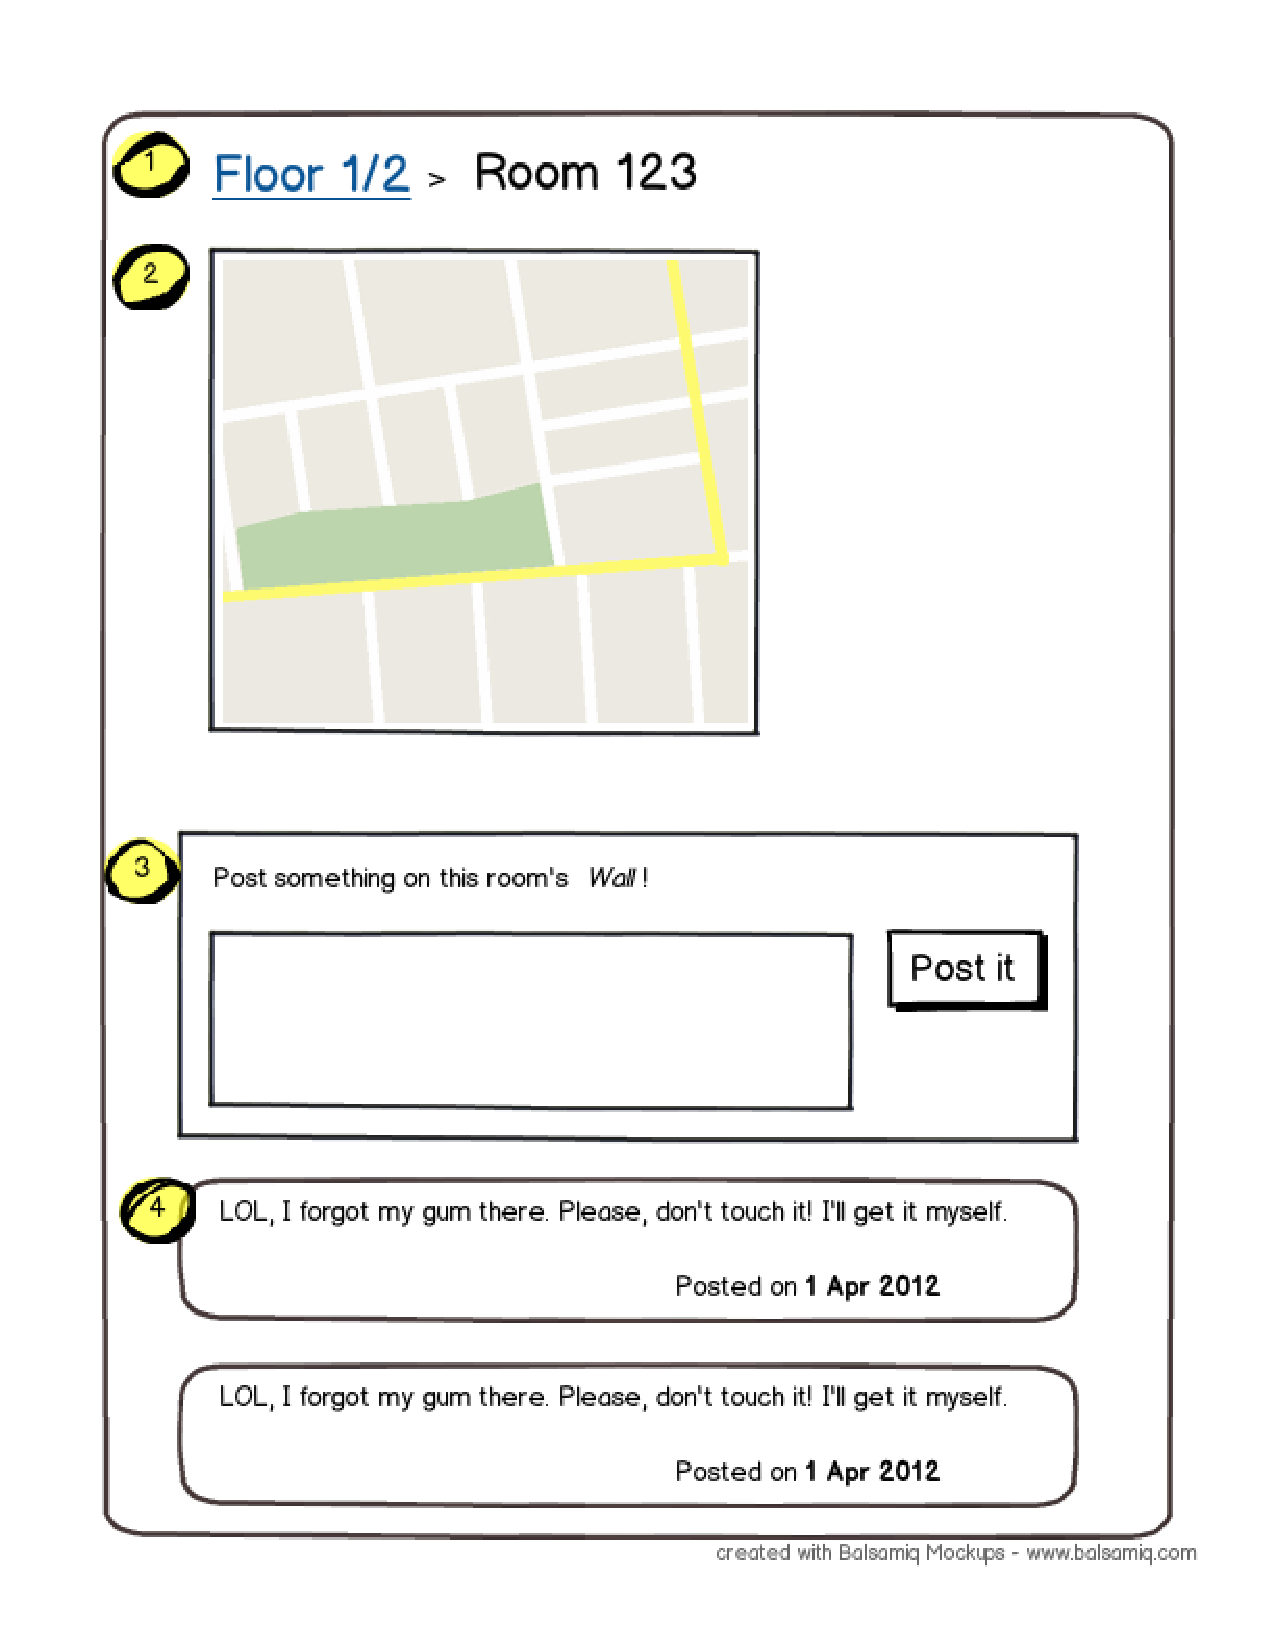
\includegraphics[scale=0.35]{img/wireframes/room.pdf}
\end{center}

The pages for \textbf{floors} are very similar to the ones for particular
\textbf{rooms} (Fig. \ref{img:wireframes-room}), the only difference being that
instead of the breadcrumbs that appear on the room page, the floor page only 
displays the floor number. The structure of these pages:
\begin{enumerate} \itemsep1pt \parskip0pt \parsep0pt
	\item{\textbf{Breadcrumbs} Level number + room number, in the case of 
	the room page.}
	\item{\textbf{Floor map} - for the room page, the particular room is
	highlighted.}
	\item{\textbf{Comment form} - small \texttt{textarea} and a 
	\texttt{Submit} button.}
	\item{\textbf{Comments} - previous comments (text + date posted)}
\end{enumerate}


\section{Application Architecture}

\subsection*{N-tier architecture}


\begin{center}
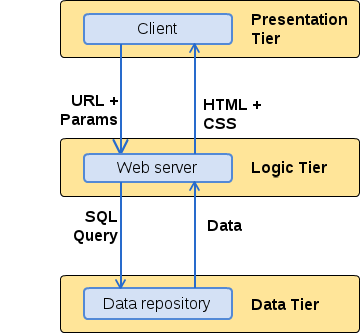
\includegraphics[scale=0.55]{img/ntier.png}
\end{center}


In order to separate data access, business logic, and presentation from each
other, we have broken our application into 3 logical tiers.

The \textbf{presentation tier} is the topmost layer of the application,
represented by the user interface. It translates user actions into commands
for the application and it presents the information retrieved by the application in a
way that the user can understand.

The \textbf{logic/application tier} is responsible for handling the requests
from the client, and making decisions regarding what information it should
retrieve from the database. It then processes and passes the received data
from the tier beneath it to the one above it.

The \textbf{data tier} is queried by the web server and it responds with the
required information.

\subsection*{ERD}

We've decided to employ a simple object to table mapping scheme to facilitate
CRUD (Create, Read, Update, Delete), operations on our data which fits in with 
our framework MVC paradigm. 

\begin{center}
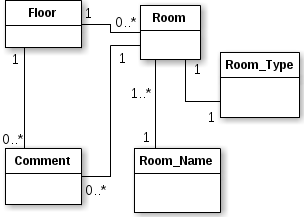
\includegraphics[scale=0.55]{img/erd.png}
\end{center}

%%%%%%%%%%%%%%%%%%%%%%%%%%%%%%%%%%%%%%%%%%%%%%%%%%%%%%%%%%%%%%%%%%%%%
% TABLE -- The floor data model + structure of the floor database %%%
%%%%%%%%%%%%%%%%%%%%%%%%%%%%%%%%%%%%%%%%%%%%%%%%%%%%%%%%%%%%%%%%%%%%%

%\begin{table}
\small{
\begin{tabular}{| p{1.8cm} | p{1cm} | p{4.2cm}|}
\hline
\multicolumn{3}{|c|}{\textbf{Floor data model}} \\
\hline
Data name & Data type & Rationale \\
\hline
id & Integer & Unique ID to identify each floor \\
\hline
description & String & Supplies extra details to optimize the search\\
\hline
date\_created & Date & The floor plan was added\\
\hline
date\_updated & Date & The floor plan was last updated\\
\hline
level & Integer & Optimize the search and reduce the fetch time\\
\hline
rating & Integer & Optimize the search by using popularity\\
\hline
GUID & Integer & Unique ID for the comment\\
\hline
\end{tabular}}	
%\caption{\small{Floor data model}}}
%\end{table}

%%%%%%%%%%%%%%%%%%%%%%%%%%%%%%%%%%%%%%%%%%%%%%%%%%%%%%%%%%%%%%%%%%%%%
\vspace{1em}
%%%%%%%%%%%%%%%%%%%%%%%%%%%%%%%%%%%%%%%%%%%%%%%%%%%%%%%%%%%%%%%%%%%%%
% TABLE -- Room data model + the structure of room database %%%%%%%%%
%%%%%%%%%%%%%%%%%%%%%%%%%%%%%%%%%%%%%%%%%%%%%%%%%%%%%%%%%%%%%%%%%%%%%

%\begin{table}
%\small{
\begin{tabular}{| p{1.8cm} | p{1cm} | p{4.2cm}|}
\hline
\multicolumn{3}{|c|}{\textbf{Room data model}} \\
\hline
Data name & Data type & Rationale \\
\hline
id & Integer & Unique ID to identify each room \\
\hline
floor\_id & Integer & FK to link the room to the floor\\
\hline
room\_name & Integer & FK to link Room\_Name\\
\hline
type & Integer & FK to link Room\_Type \\
\hline
description & String & Information about the room\\
\hline
rating & Integer & Optimize the search by using popularity\\
\hline
GUID & Integer & Unique ID for the comment\\
\hline
\end{tabular}	
%\caption{\small{Room data model}}}
%\end{table}

%%%%%%%%%%%%%%%%%%%%%%%%%%%%%%%%%%%%%%%%%%%%%%%%%%%%%%%%%%%%%%%%%%%%%
\vspace{1em}
%%%%%%%%%%%%%%%%%%%%%%%%%%%%%%%%%%%%%%%%%%%%%%%%%%%%%%%%%%%%%%%%%%%%%
% TABLE -- Comment data model + the structure of comment database %%% 
%%%%%%%%%%%%%%%%%%%%%%%%%%%%%%%%%%%%%%%%%%%%%%%%%%%%%%%%%%%%%%%%%%%%%

%\begin{table}
%\small{
\begin{tabular}{| p{1.8cm} | p{1cm} | p{4.2cm}|}
\hline
\multicolumn{3}{|c|}{\textbf{Comment data model}} \\
\hline
Data name & Data type & Rationale \\
\hline
GUID & Integer & Unique ID for the comment\\
\hline
comment & String & The content of the comment\\
\hline
date & Date & The comment was posted\\
\hline
\end{tabular}	
%\caption{\small{Comment data model}}}
%\end{table}

%%%%%%%%%%%%%%%%%%%%%%%%%%%%%%%%%%%%%%%%%%%%%%%%%%%%%%%%%%%%%%%%%%%%%
%%%%%%%%%%%%%%%%%%%%%%%%%%%%%%%%%%%%%%%%%%%%%%%%%%%%%%%%%%%%%%%%%%%%%
\vspace{1em}
%%%%%%%%%%%%%%%%%%%%%%%%%%%%%%%%%%%%%%%%%%%%%%%%%%%%%%%%%%%%%%%%%%%%%
% TABLE - Room_Type data model + the structure of room_type database%
%%%%%%%%%%%%%%%%%%%%%%%%%%%%%%%%%%%%%%%%%%%%%%%%%%%%%%%%%%%%%%%%%%%%%

%\begin{table}
%\small{
\begin{tabular}{| p{1.8cm} | p{1cm} | p{4.2cm}|}
\hline
\multicolumn{3}{|c|}{\textbf{Room\_Type data model}} \\
\hline
Data name & Data type & Rationale \\
\hline
type\_id & Integer & Unique ID \\
\hline
type & String & Type of the room (e.g. lab, lecture theatre, etc.)\\
\hline
\end{tabular}	
%\caption{\small{Room\_Type data model}}}
%\end{table}

%%%%%%%%%%%%%%%%%%%%%%%%%%%%%%%%%%%%%%%%%%%%%%%%%%%%%%%%%%%%%%%%%%%%%
\vspace{1em}
%%%%%%%%%%%%%%%%%%%%%%%%%%%%%%%%%%%%%%%%%%%%%%%%%%%%%%%%%%%%%%%%%%%%%
% TABLE - Room_Name data model + the structure of room_name database%
%%%%%%%%%%%%%%%%%%%%%%%%%%%%%%%%%%%%%%%%%%%%%%%%%%%%%%%%%%%%%%%%%%%%%

%\begin{table}
%\small{
\begin{tabular}{| p{1.8cm} | p{1cm} | p{4.2cm}|}
\hline
\multicolumn{3}{|c|}{\textbf{Room\_name data model}} \\
\hline
Data name & Data type & Rationale \\
\hline
room\_id & Integer & FK refencing Room.room\_id \\
\hline
name & String & Name of the room \\
\hline
\end{tabular}	
%\caption{\small{Room\_Name data model}}}
%\end{table}

%%%%%%%%%%%%%%%%%%%%%%%%%%%%%%%%%%%%%%%%%%%%%%%%%%%%%%%%%%%%%%%%%%%%%
%%%%%%%%%%%%%%%%%%%%%%%%%%%%%%%%%%%%%%%%%%%%%%%%%%%%%%%%%%%%%%%%%%%%%


\section{Message Passing}


(Figure \ref{img:diagram-sequence}):

WhereInTheBob is a fully standards compliant web application.
Since our requirenments are fairly standard , a mix of openly supported 
technologies will be employed:

\begin{itemize}
\item \textbf{ Client to Server } requests and responses are HTTP.
\\ A mix of POST and GET requests will be employed. 
	\begin{itemize}
		\item \textbf{POST} requests will be used for sensitive data such as "Username" and "Password" strings
	to avoid leaving personally identifiable information behind in places
	such as the browser's url history.
		\item \textbf{GET} requests with parameters will be used in the "floor" and "room" lookup
	requests. 
	\end{itemize}

\item \textbf{Server to Data Store } communications will be handled trough standards SQL queries.
The underlying protocol will differ in our development and production servers
as SQLite is easier to use in a development environment (local api calls ). \\
\\
In an production environment however the standard MySql connection protocol will
be used.
\end{itemize}
Our chose framework , DjAngo supports all of these technologies and protocols
natively. The protocols themselves are wildly popular and so we will not discuss
them any further.

\begin{center}
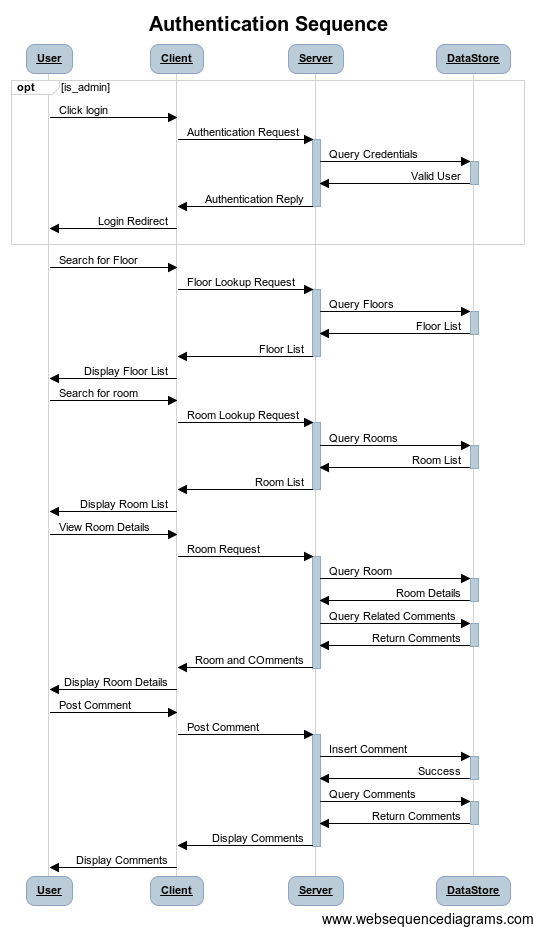
\includegraphics[scale=0.35]{img/dia.png}
\end{center}

\section{Summary and Future Work}
\begin{itemize}\itemsep1pt \parskip0pt \parsep0pt
\item	Summary of application and its current state.
\item	A list or table of all the technologies, standards, and protocols that will be required.
\item	A short description of the limitations imposed concerning development.
\item   A summary of future development.
\end{itemize}

\section{Acknowledgements}
Our thanks to the lecturers and demonstrators for their comments and suggestions. 
And our thanks to the peer reviewers for their feedback. 

\bibliographystyle{abbrv}
\bibliography{sig-proc}

%\section{Appendix}
%\newpage
%\begin{figure}
\begin{minipage}[b]{0.5\linewidth}\centering
        % \begin{center}
                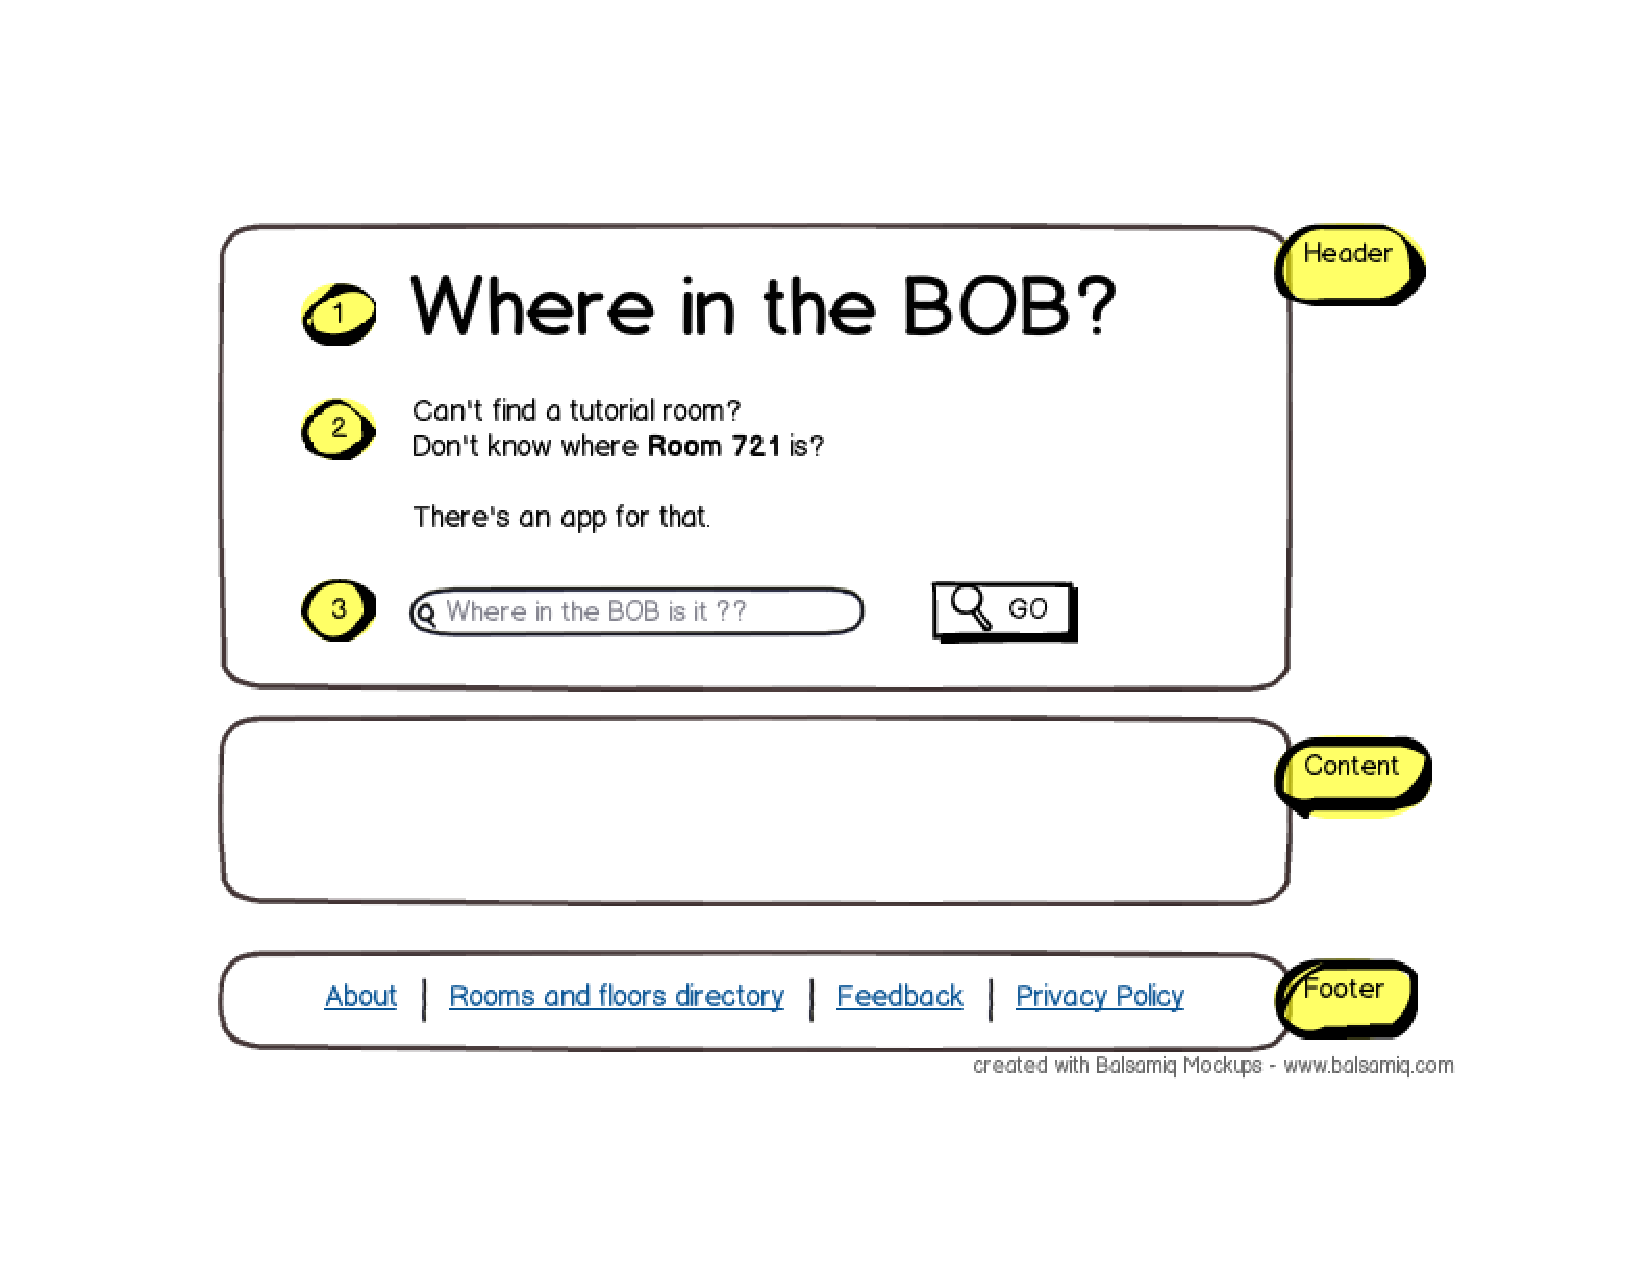
\includegraphics[scale=0.35]{img/wireframes/home.pdf}
                \caption{Wireframe for the Home page.}
                \label{img:wireframes-home}
        % \end{center}
\end{minipage}
%\end{figure}
%\begin{figure}
\hspace{4cm}
\begin{minipage}[b]{0.5\linewidth}\centering
        % \begin{center}
                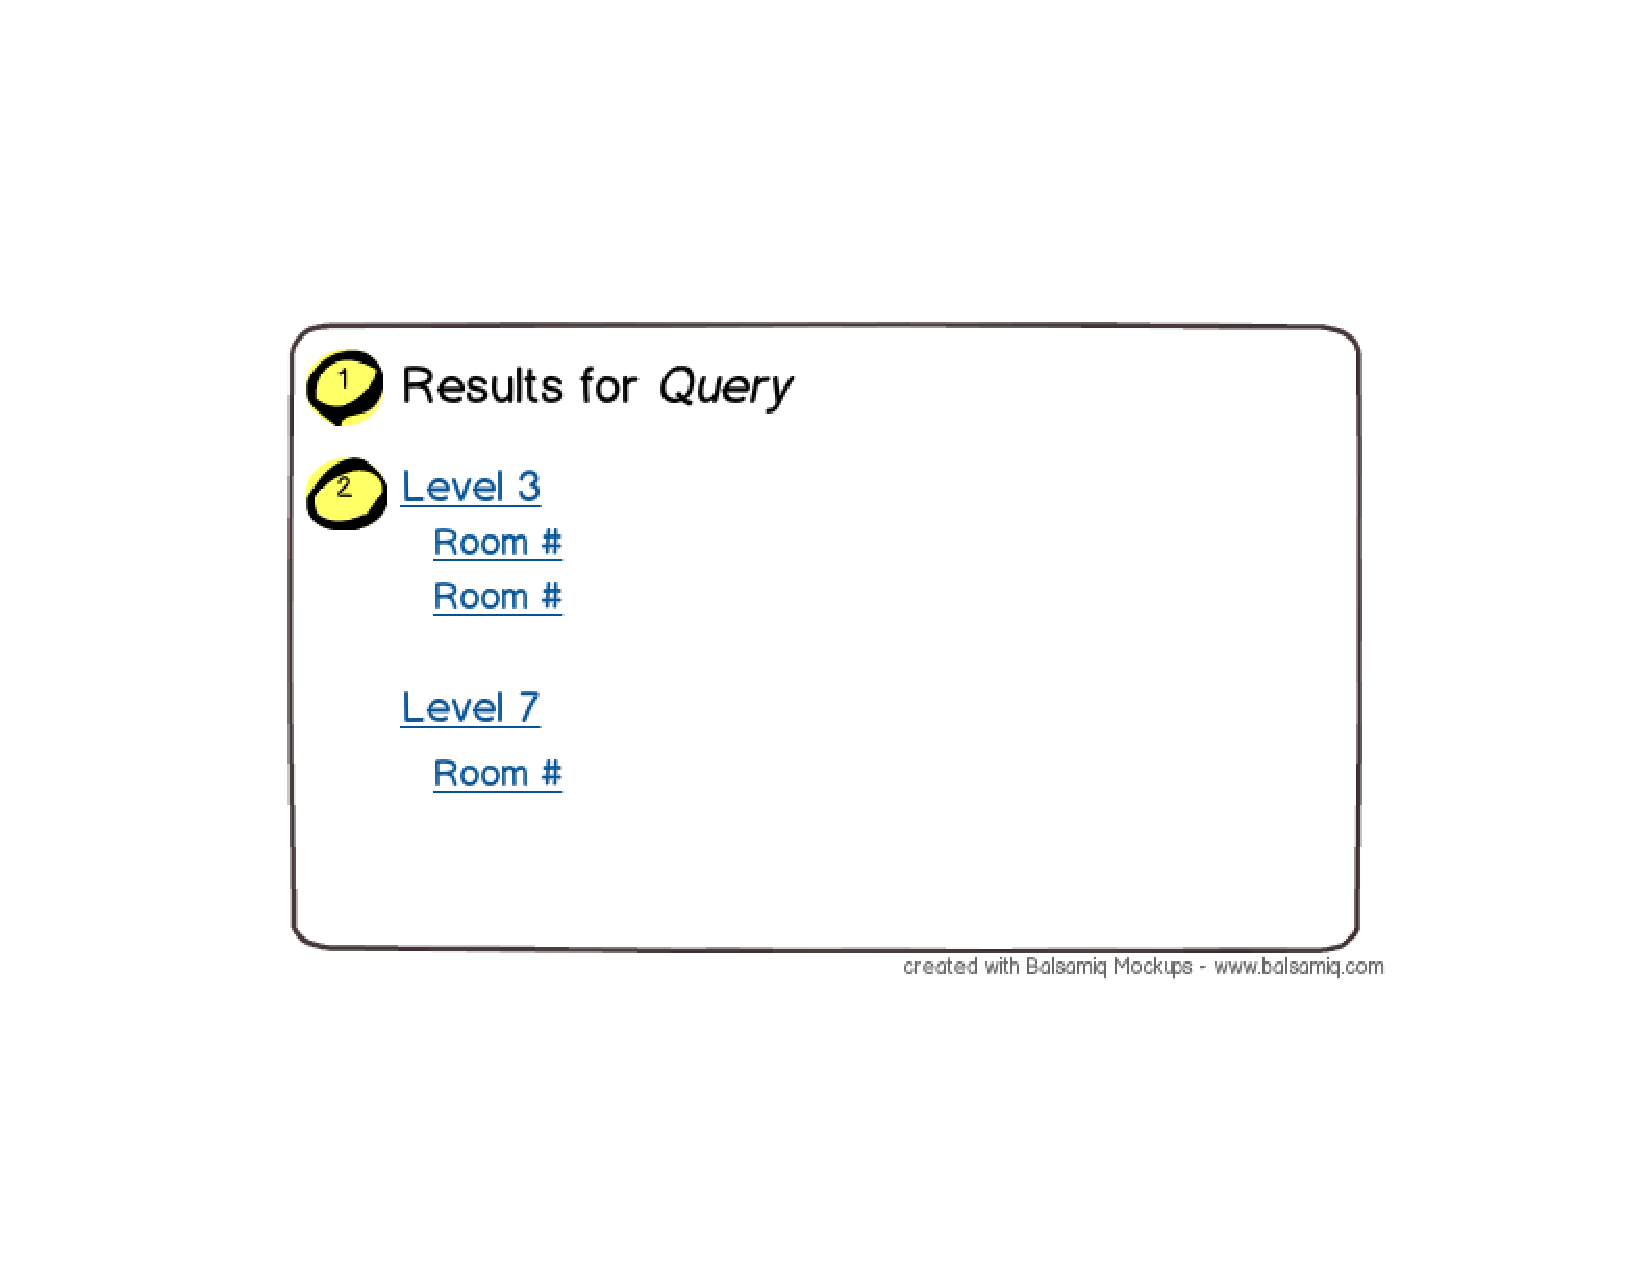
\includegraphics[scale=0.35]{img/wireframes/results.pdf}
                \caption{Wireframe for the Results/Directory page.}
                \label{img:wireframes-results}
        % \end{center}
\end{minipage}
\end{figure}


%\begin{figure}
%\begin{minipage}[b]{0.5\linewidth}\centering
        % \begin{center}
%                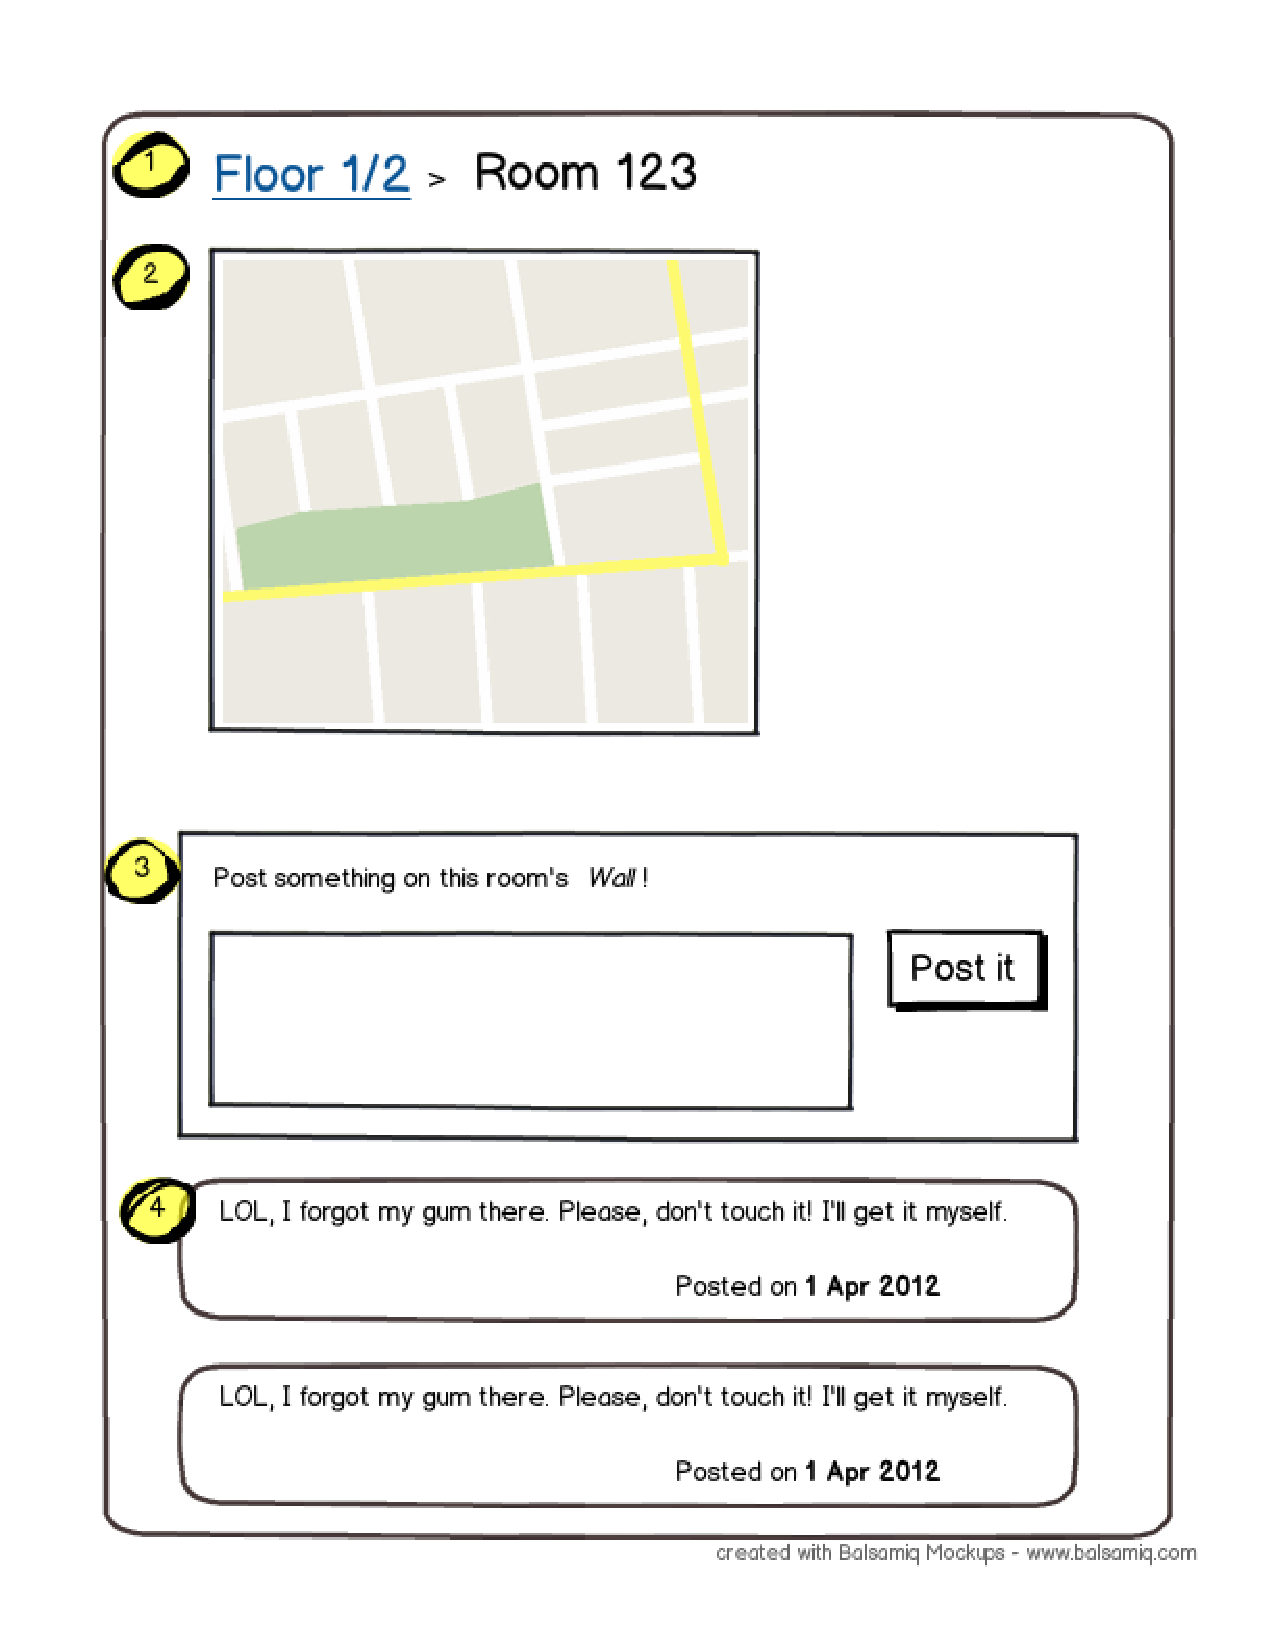
\includegraphics[scale=0.35]{img/wireframes/room.pdf}
%                \caption{Wireframe for the Room/Floor page.}
%                \label{img:wireframes-room}
        % \end{center}
%\end{minipage}
%\end{figure}
%\begin{figure}
%\hspace{4cm}

%\begin{minipage}[b]{0.5\linewidth}\centering

        % \begin{center}
%                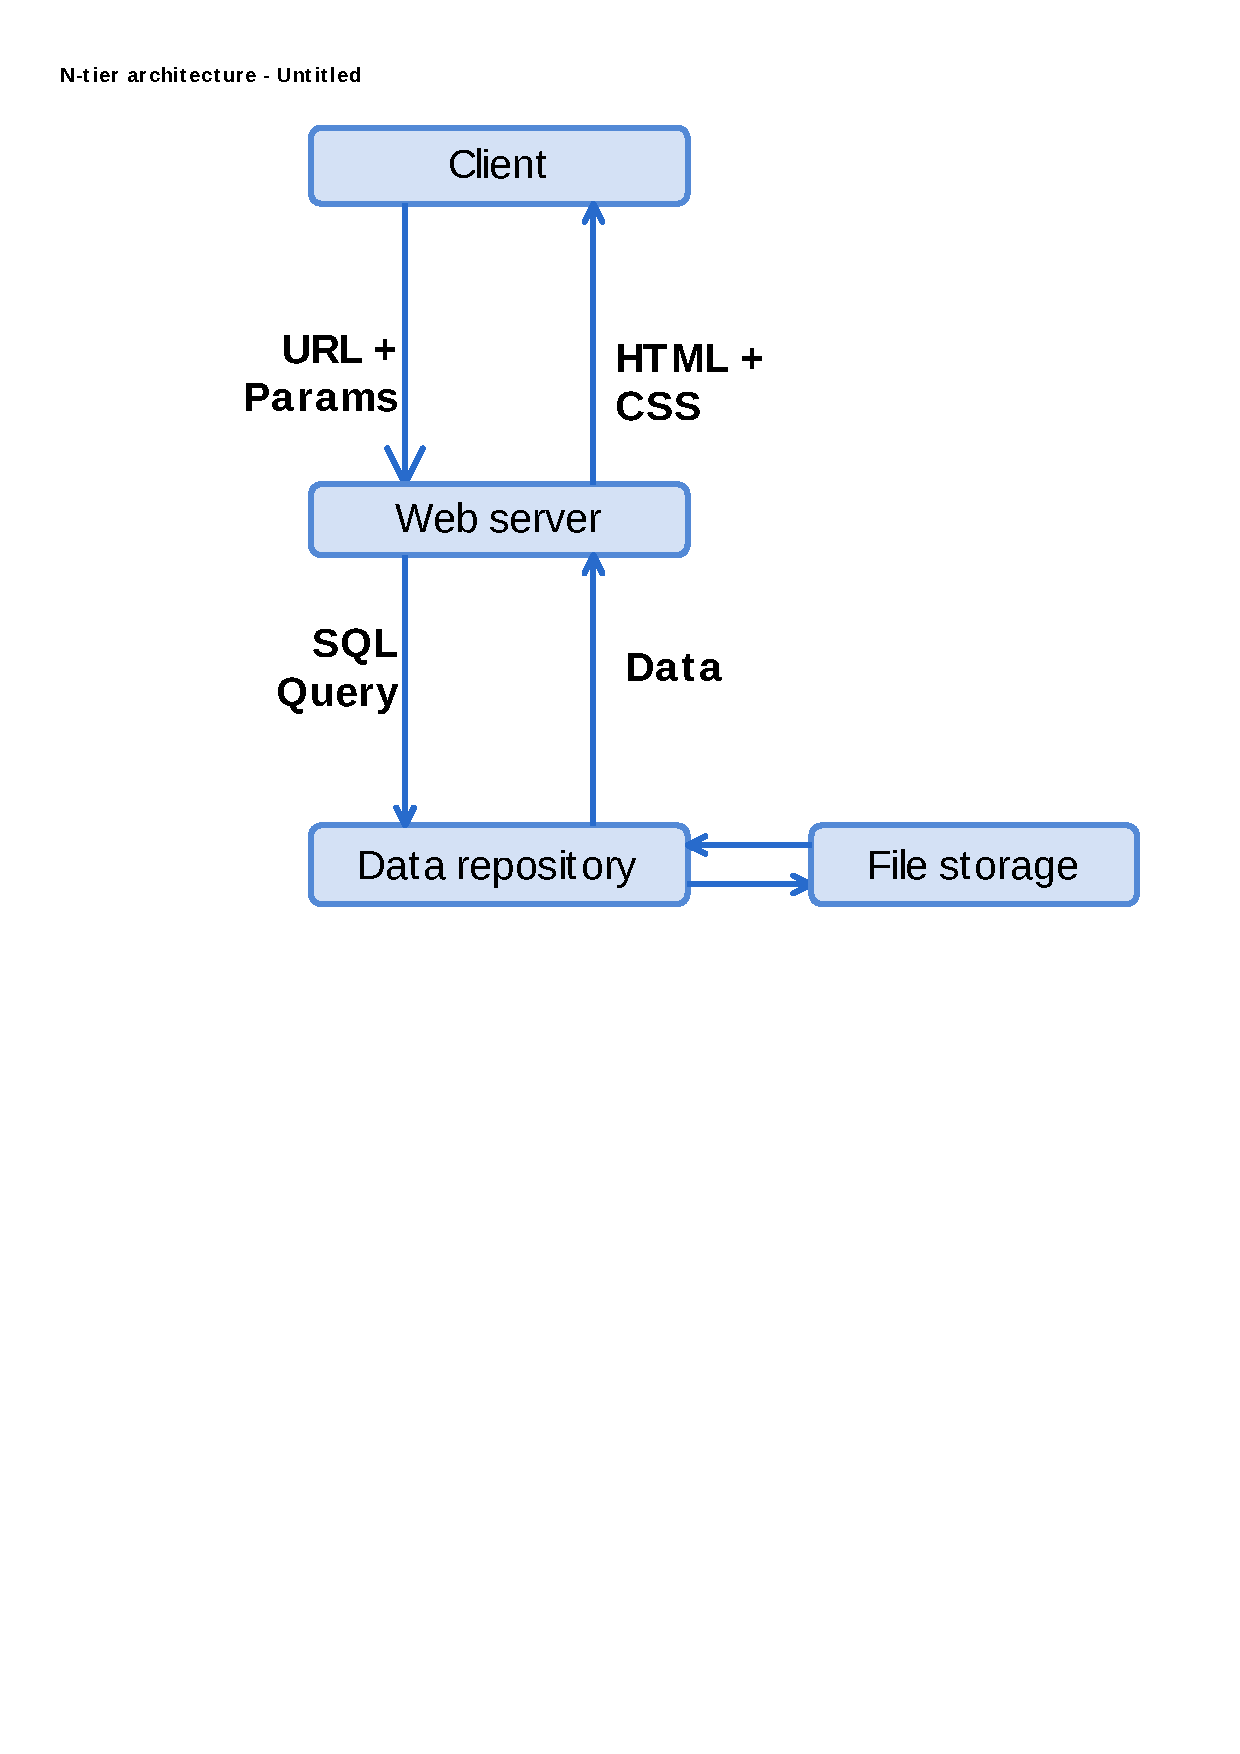
\includegraphics[scale=0.35]{img/ntier.pdf}
%                \caption{N-tier architecture.}
%                \label{img:arch-ntier}
        % \end{center}
%\end{minipage}
%\end{figure}
%\begin{figure}
        % \begin{center}
                % 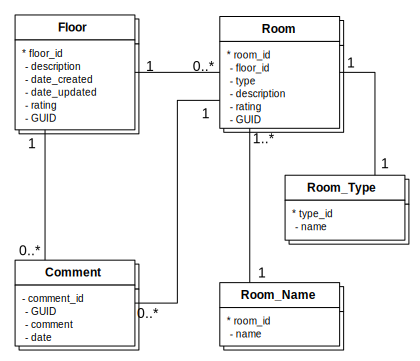
\includegraphics[scale=0.35]{img/erd.pdf}
%                \caption{ERD.}
%                \label{img:arch-ntier}
        % \end{center}
%\end{figure}
%\begin{figure}
        % \begin{center}
%                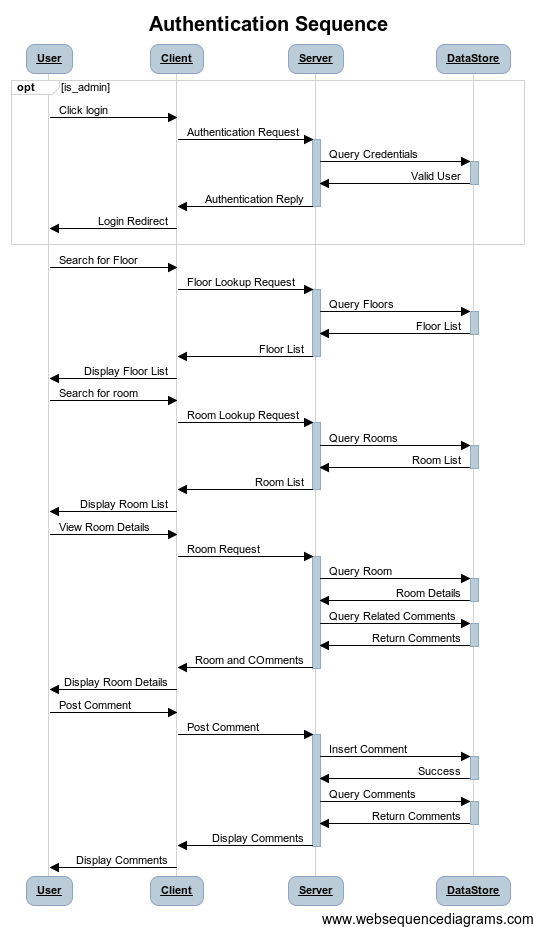
\includegraphics[scale=0.35]{img/dia.png}
%                \caption{Sequence Diagram.}
%                \label{img:diagram-sequence}
        % \end{center}
%\end{figure}


\end{document}
